\documentclass{report}

% Packages for images.
\usepackage{graphicx}
\usepackage{float}

% Packages for mathematical formulae/symbols.
\usepackage{amsmath}
\usepackage{amssymb}
\usepackage{amsfonts}

% Packages for code snippets and algorithms.
\usepackage{listings}
\usepackage{xcolor}
\definecolor{codegreen}{RGB}{0,128,0}
\definecolor{codegray}{RGB}{110,110,110}
\definecolor{codepurple}{RGB}{163,21,21}
\definecolor{codeblue}{RGB}{0,0,180}
\definecolor{backwhite}{RGB}{255,255,255}
\definecolor{backcolour}{RGB}{248,248,248}
\lstdefinestyle{mypython}{
    language=Python,
    backgroundcolor=\color{backwhite},
    basicstyle=\ttfamily\small,
    keywordstyle=\color{codeblue}\bfseries,
    commentstyle=\color{codegreen}\itshape,
    stringstyle=\color{codepurple},
    numberstyle=\tiny\color{codegray},
    numbers=left,
    numbersep=8pt,
    frame=single,
    rulecolor=\color{black!20},
    breaklines=true,
    showstringspaces=false,
    tabsize=4,
    keepspaces=true
}
\lstset{style=mypython}
\usepackage[ruled,vlined]{algorithm2e}

% Creating the Example boxes.
\definecolor{exampleback}{RGB}{240, 248, 240}
\definecolor{exampleframe}{RGB}{34, 112, 62}
\usepackage[most]{tcolorbox}
\newtcolorbox{examplebox}[1][]{
    colback=exampleback,
    colframe=exampleframe,
    coltitle=white,
    fonttitle=\bfseries,
    title={Example\ifblank{#1}{}{: #1}},
    arc=2pt,
    boxrule=1pt
}

% Packages for styling and layout.
\usepackage{booktabs}
\usepackage{array}
\usepackage{geometry}
\usepackage{hyperref}

% Packages for plotting graphs.
\usepackage{tikz}
\usepackage{pgfplots}
\pgfplotsset{compat=1.18}

% Packages for compilation.
\usepackage{microtype}

\begin{document}

\begin{titlepage}
    \centering
    \vspace*{2cm}
    
    % Subject Title.
    {\Huge \bfseries Algorithmic Methods of Data Mining and Laboratory \par}
    \vspace{1.5cm}
    
    % Master's Degree and Faculty.
    {\Large Master's Degree in Data Science, Sapienza Università di Roma \par}
    {\large Faculty of Information Engineering, Informatics and Statistics \par}
    \vspace{0.5cm}
    
    % Department.
    {\large Department of Computer Science \par}
    \vspace{3cm}
    
    % Author.
    {\Large \textbf{Author:} Gianmaria Romano \par}
    \vspace{3cm}

    % Reference Bibliography
    {\Large Reference Bibliography \par}
    {\large C. Aggarwal: \href{https://www.charuaggarwal.net/Data-Mining.htm}{\textit{Data Mining: The Textbook}} \\
    R. Zafarani, M. A. Abbasi, and H. Liu: \href{https://dmml.asu.edu/smm/}{\textit{Social Media Mining: An Introduction}} \\
    J. Leskovec, A. Rajaraman, and J. Ullman: \href{http://www.mmds.org/}{\textit{Mining of Massive Datasets}} \\
    C. D. Manning, P. Raghavan, and H. Schütze: \href{https://www-nlp.stanford.edu/IR-book/}{\textit{Introduction to Information Retrieval}} \\
    J. Janssens: \href{https://github.com/jeroenjanssens/data-science-at-the-command-line}{\textit{Data Science at the Command Line}} \\}
    \vfill
    
    % Academic Year.
    {\large Academic Year 2026/2027 \par}
    \vspace*{1cm}
\end{titlepage}

\clearpage

%\maketitle
\begin{tcolorbox}[colback=gray!5!white, colframe=gray!75!black, title=Disclaimer]
    This document contains notes for the \textbf{Algorithmic Methods of Data Mining and Laboratory} course, given by \textbf{Professors Anagnastopolous and Siciliano} as part of the Master’s Degree in Data Science at \textbf{Sapienza Università di Roma} during the \textbf{first} semester of Academic Year \textbf{2026/2027}.
    
    \smallskip
    \textbf{Note: }These notes may not cover all details of each lecture, so it is highly suggested to consult the Professor's official resources and materials. 
    
    \smallskip
    \textbf{Important: }These notes are free to share and use, but please remember to credit me as the author and do not try to hide/remove this page.
\end{tcolorbox}

\begin{tcolorbox}[colback=gray!5!white, colframe=gray!75!black, title=Contacts]
    For further information or requests, feel free to \href{https://t.me/toritosenso}{contact me privately} or reach out through my repository: \href{https://github.com/GianmariaRomano/Data-Science-Notes}{https://github.com/GianmariaRomano/Data-Science-Notes}.
\end{tcolorbox}

\begin{tcolorbox}[colback=gray!5!white, colframe=gray!75!black, title=License]
    These documents are distributed under the \href{https://www.gnu.org/licenses/gpl-3.0.en.html}{GNU General Public License 3.0}, a form of copyleft intended for use on a manual, textbook or other documents. Material licensed under the current version of the license can be used for any purpose, as long as the use meets certain conditions:
    \begin{itemize}
        \item All previous authors of the work must be attributed.
        \item All changes to the work must be logged.
        \item All derivative works must be licensed under the same license.
        \item The full text of the license, unmodified invariant sections as defined by the author if any, and any other added warranty disclaimers (such as a general disclaimer alerting readers that the document may not be accurate for example) and copyright notices from previous versions must be maintained.
        \item Technical measures such as DRM may not be used to control or obstruct distribution or editing of the document.
    \end{itemize}
\end{tcolorbox}

\tableofcontents

\chapter{Introduction to data mining}
\section{Finding a definition of data mining}
While no unique definition exists yet, it is possible to view data mining as the use of efficient techniques for the analysis of very large collections of data and the extraction of useful and possibly unexpected patterns in data in order to make decisions across various areas.
\begin{examplebox}[Descriptive and predictive data mining]
    Descriptive data mining aims to identify patterns and relationships within data using unsupervised learning techniques that can be applied to recommendation systems, such as Netflix or Spotify's engines, to analyse patterns in user behaviour. \newline
    On the other hand, predictive data mining focuses on using past observations to predict a target variable through supervised learning techniques. \newline
    For instance, CERN's \textit{A Large Ion Collided Experiment} analyses heavy-ion collision data to investigate the properties of quark-gluon plasma.
\end{examplebox}
\section{Understanding data types}
Since data can come in different forms, it is necessary to organize it in order to extract meaningful information or patterns. \newline
In particular, data can be seen as a collection of attributes that describe some objects and, depending on the organization paradigm, data can be classified into three main types:
\begin{itemize}
    \item \textbf{Structured data: }Data is organized according to a well-defined schema that is enforced during storage.
    \item \textbf{Semi-structured data: }Data can be organized according to a structural schema, although this organization paradigm may not be enforced during storage.
    \item \textbf{Unstructured data: }Data does not follow a pre-defined structure, requiring a data cleaning procedure to store it as (semi-)structured data before use.
\end{itemize}
\begin{examplebox}[Different data types]
    Examples of data organization can be seen on the InfoStud platform, which enforces strict organization through dedicated constraints on certain types of data, and medical records, which follow some structural patterns but might contain errors or anomalous data. \newline
    By contrast, social media platforms, such as Twitter or Reddit, provide clear examples of unstructured data that do not follow an organizational structure.
\end{examplebox}
\subsection{Numeric data}
If each record has the same fixed set of numeric attribute, it can be seen as a point in a multi-dimensional space, meaning that the dataset can be treated as a matrix.
\begin{figure}[H]
    \centering
    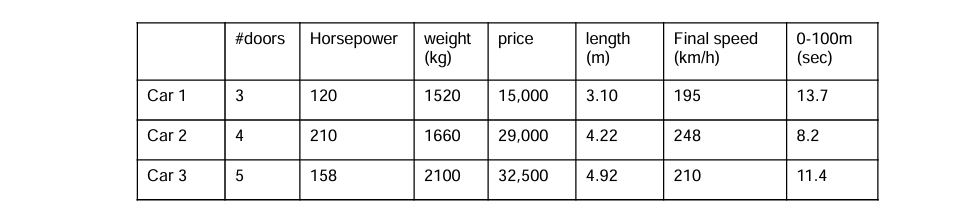
\includegraphics[width=0.4\linewidth]{images/numeric_data.png}
    \caption{Example of numeric record data.}
    \label{fig:numeric_data}
\end{figure}
\subsection{Categorical data}
Categorical data consists of a collection of records with a fixed set of categorical variables.
\begin{figure}[H]
    \centering
    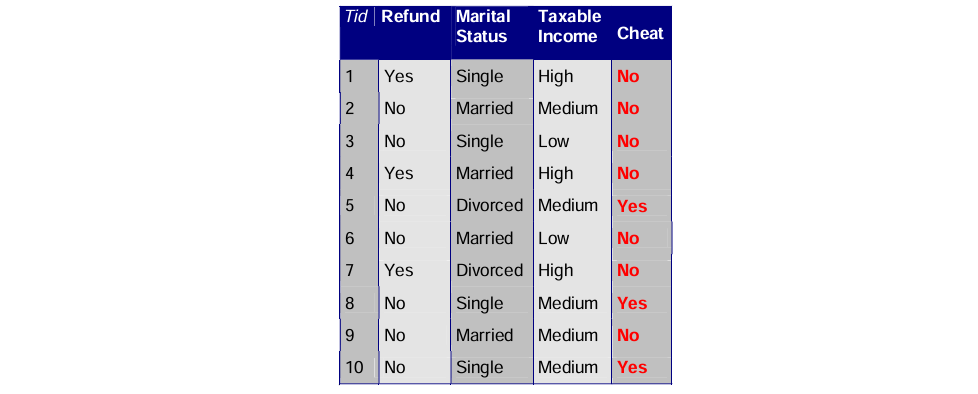
\includegraphics[width=0.4\linewidth]{images/categorical_data.png}
    \caption{Example of categorical record data.}
    \label{fig:categorical_data}
\end{figure}
\subsection{Document data}
Using the ``bag-of-words'' representation, a document can be represented using a text vector that indicates the occurrences of certain words of interest within the document.
\begin{figure}[H]
    \centering
    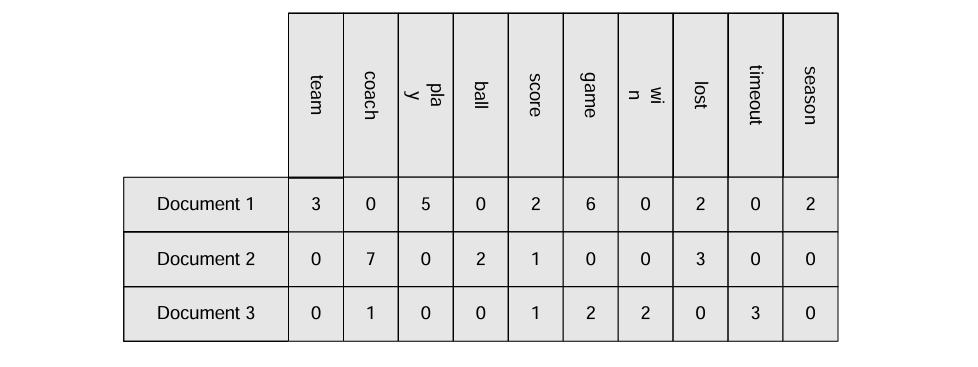
\includegraphics[width=0.4\linewidth]{images/document_data.png}
    \caption{Example of document data.}
    \label{fig:document_data}
\end{figure}
\noindent However, text vectors are often vulnerable to the ``curse of dimensionality'', which denotes all the performance problems that arise when dealing with high-dimensional data. \newline
For this reason, document data are often pre-processed using dimensionality reduction techniques or principal component analysis in order to focus on just the relevant information carried by the data.
\subsection{Set data}
Set data can be seen as an efficient way of representing collections through binary attributes.
\begin{figure}[H]
    \centering
    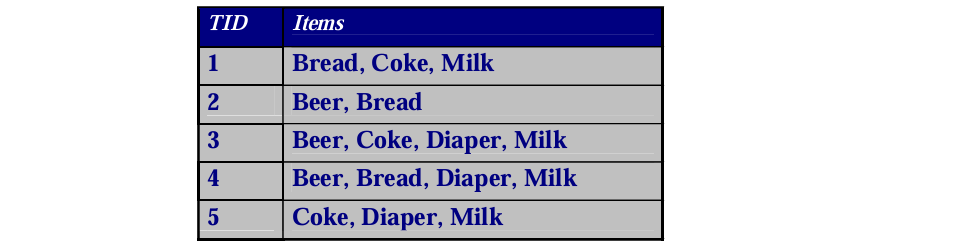
\includegraphics[width=0.4\linewidth]{images/set_data.png}
    \caption{Example of set data.}
    \label{fig:set_data}
\end{figure}
\noindent Note that this type of data is often used to compress document data into sets of words.
\subsection{Ordered data}
Ordered data consists of ordered sequences of values that come in handy for genomics or for time-series forecasting.
\subsection{Graph data}
Graph data allows to summarise web network data using a (directed) graph $\displaystyle G(V, E)$ whose nodes represent pages or users and whose edges denote connections, such as links or interactions, between pages or users.
\section{Storing data}
A computer typically features a processor that performs calculations on data that can be stored on its memory or on (external) hard disks. \newline
Most of the time, however, data is stored using a cloud infrastructure that consists of clustered server racks that can store large amounts of data that might not fit on a normal computer.

\chapter{Algorithms}
\section{Defining algorithms}
An algorithm can be seen as a set of instructions to solve a given problem. \newline
In particular, an algorithm is evaluated based on its correctness, which determines whether the algorithm works on every possible input or not, and its efficiency, which measures the time taken by the algorithm to find a solution to the given problem.
\begin{examplebox}[The maximum value of an array]
    Consider an algorithm that finds the maximum value in an array of $\displaystyle n$ elements:
    \begin{algorithm}[H]
        \caption{Finding the Maximum Value in an Array.}
        \KwData{An array $\displaystyle A$ of size $\displaystyle n$}
        \KwResult{$\displaystyle \max(A)$}
    
        $m \gets A[1]$\;
        \For{$i \gets 1$ \KwTo $n$}{
            \If{$A[i] > m$}{
                $m \gets A[i]$\;
            }
        }
        \Return{$m$}\;
    \end{algorithm}
    \noindent The correctness of this algorithm can be proved by induction on the number of steps.
    \begin{itemize}
        \item For the base case, given by $\displaystyle k = 1$, $\displaystyle A[k]$ is trivially the maximum value.
        \item Assuming the algorithm is correct on an input of size $\displaystyle k$, the goal is to prove its correctness on an input of size $\displaystyle (k + 1)$ as well. \newline
        Claim that, after $\displaystyle k$ steps, $\displaystyle m = \max_{i \in \{1, \dots, k\}}(A[i])$: it is possible to see that $\displaystyle m$ will be updated if and only if $\displaystyle A[k + 1] > m$.
    \end{itemize}
    Additionally, looking at the pseudocode allows to bound the running time of this algorithm to at most $\displaystyle 3n + 2$ moves on an input of size $\displaystyle n$.
\end{examplebox}
\noindent Generally speaking, an algorithm is written using pseudocode in order to provide a language-independent idea of the solution to the given problem.
\section{Complexity analysis}
The running time of an algorithm is a function $\displaystyle T(n)$ that describes the number of steps done by the algorithm to solve a problem on an input of size $\displaystyle n$. \newline
Since algorithm efficiency often depends on the code or machine that is used, it is often sufficient to find an estimate of the running time of an algorithm through asymptotic analysis. \newline
\begin{figure}[H]
    \centering
    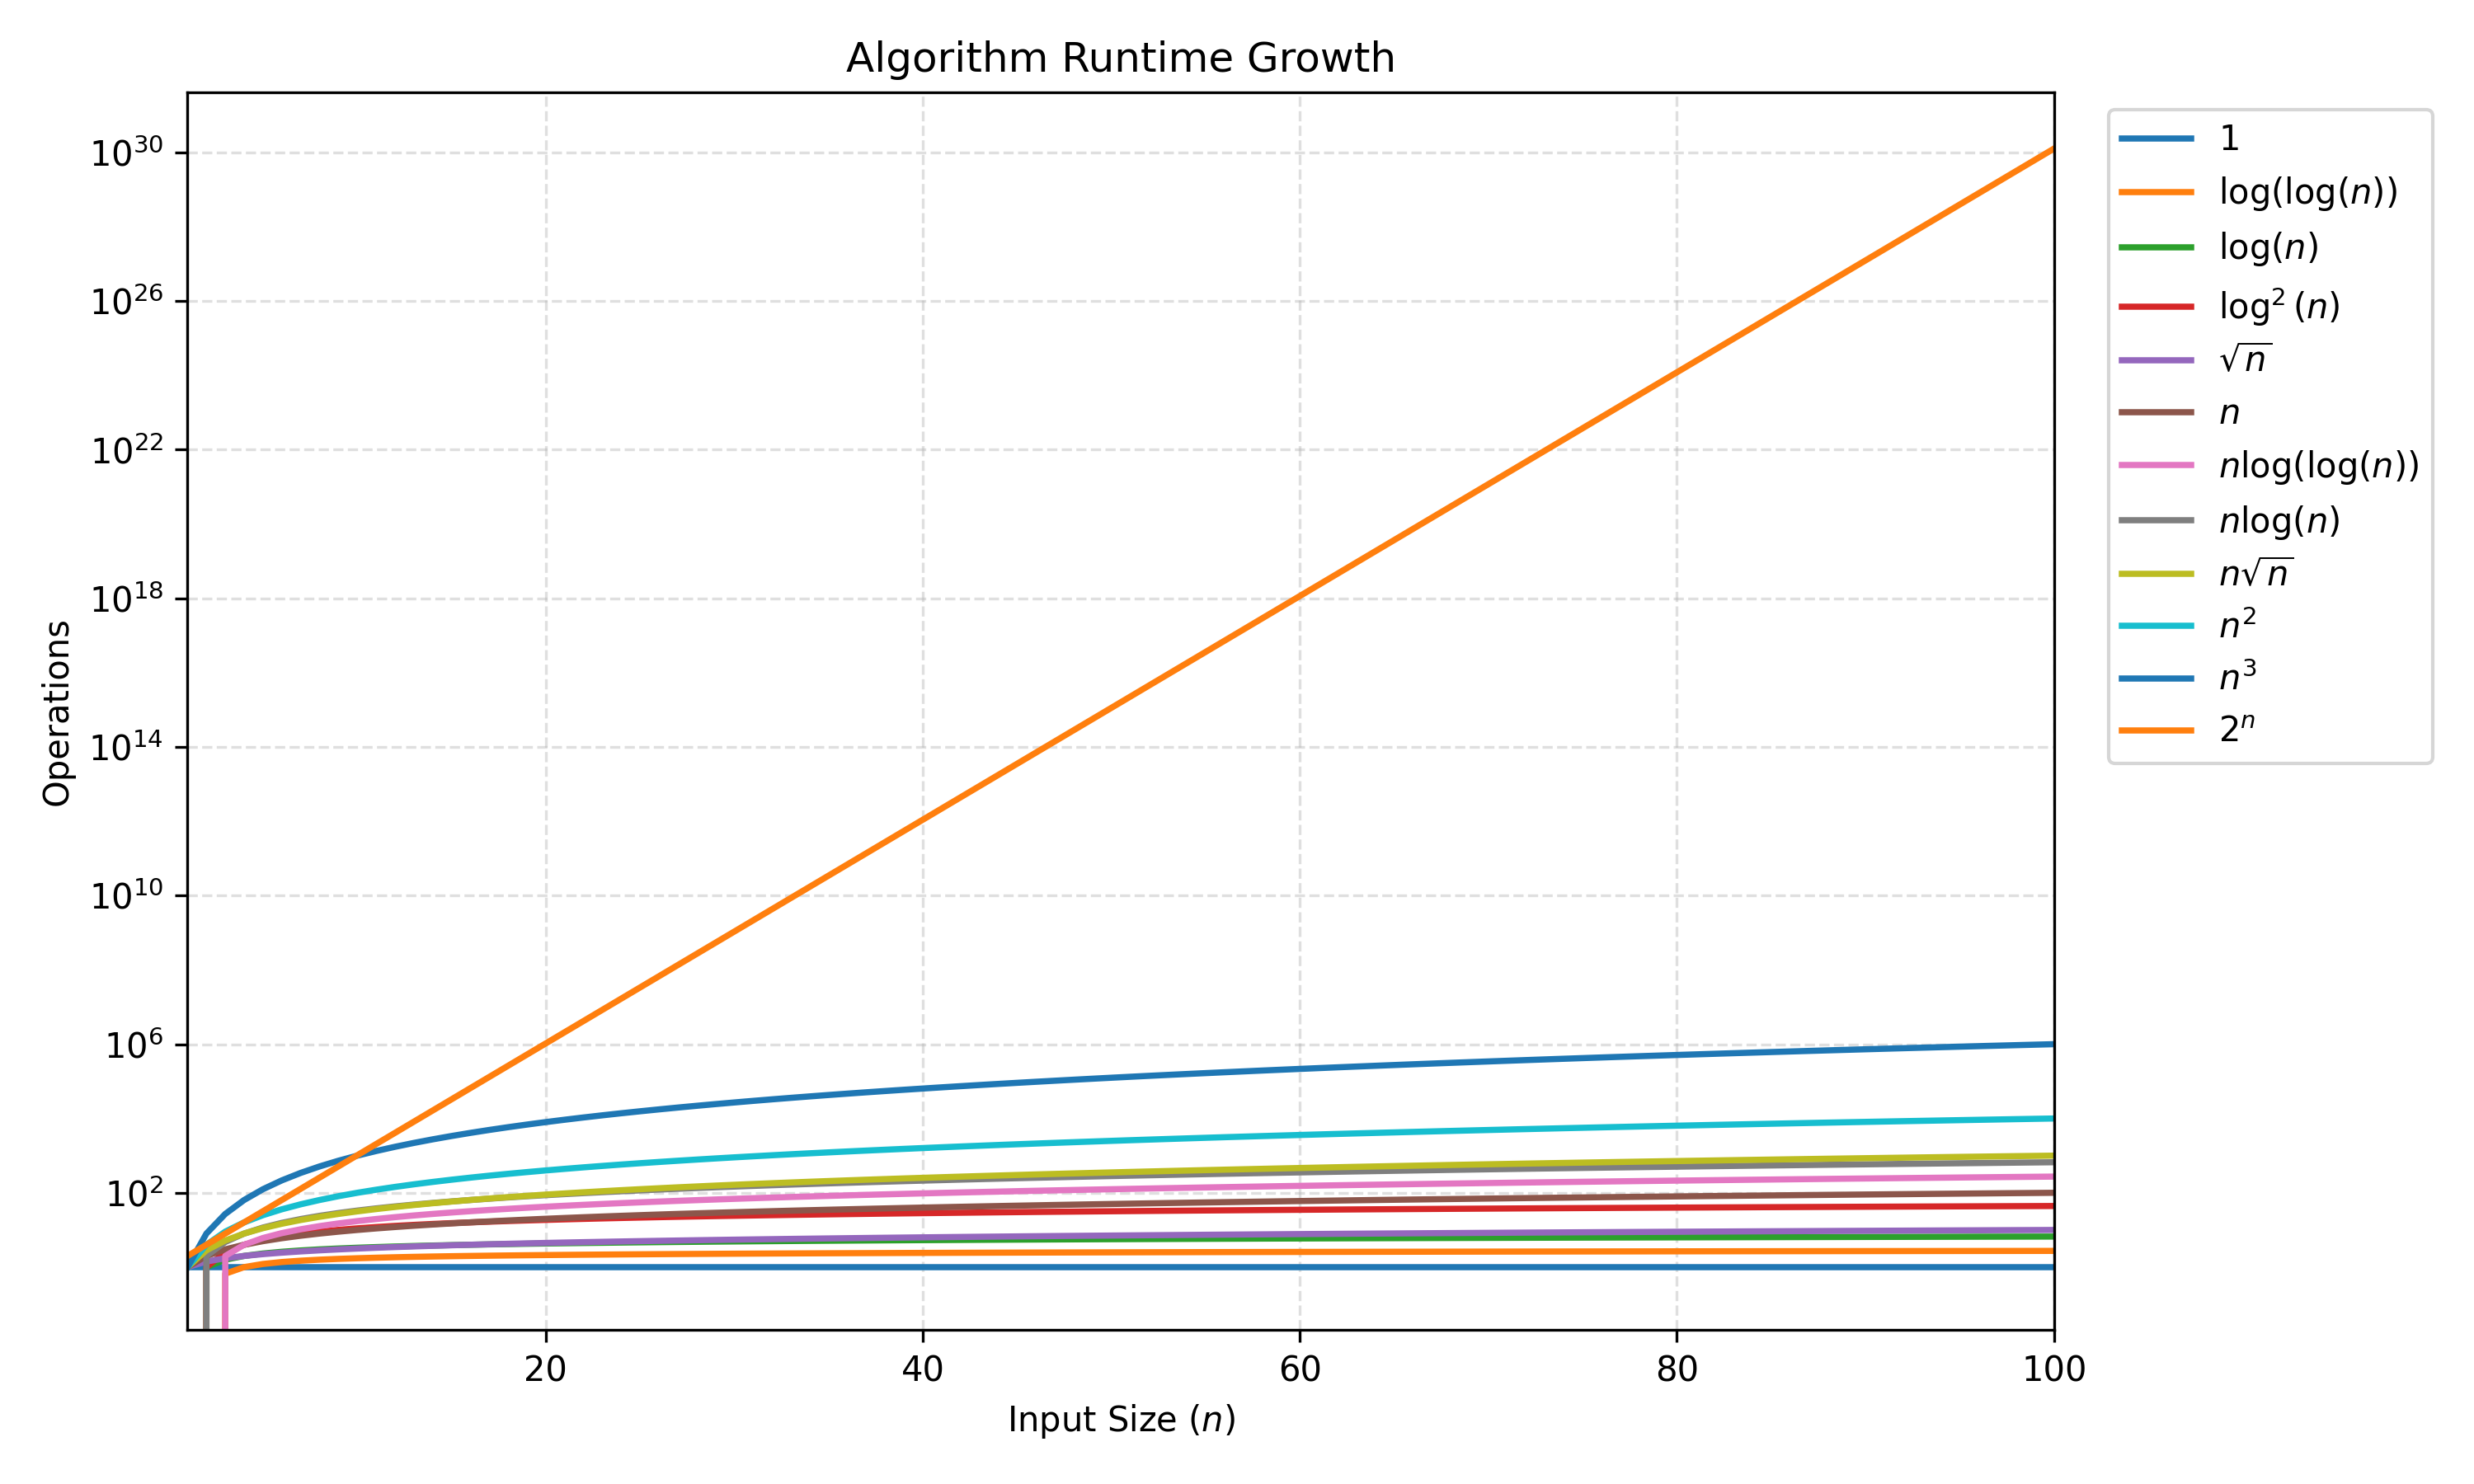
\includegraphics[width=0.75\linewidth]{images/complexities.png}
    \caption{Visual comparison of common running time growth rates.}
    \label{fig:complexity}
\end{figure}
\noindent Therefore, given a function $\displaystyle g: \mathbb{N} \to \mathbb{R}^+$, it is possible to define the following asymptotic bounds:
\begin{itemize}
    \item \textbf{Upper bound: }$\displaystyle T(n) = O(g(n))$ if it is possible to find $\displaystyle c > 0$ and $\displaystyle n_0 \ge 0$ such that
    \[0 \leq T(n) \leq c \cdot g(n) \text{ } \forall n \ge n_0\]
    \item \textbf{Lower bound: }$\displaystyle T(n) = \Omega(g(n))$ if it is possible to find $\displaystyle c > 0$ and $\displaystyle n_0 \ge 0$ such that
    \[0 \leq c \cdot g(n) \leq T(n) \text{ } \forall n \ge n_0\]
    \item \textbf{Tight bound: }$\displaystyle T(n) = \Theta(g(n))$ if it possible to find $\displaystyle c_1, c_2 > 0$ and $\displaystyle n \ge n_0$ such that
    \[0 \leq c_1 \cdot g(n) \leq T(n) \leq c_2 \cdot g(n) \text{ } \forall n \ge n_0\]
\end{itemize}
\begin{examplebox}[The prefix sum problem] % DA FINIRE
    The following algorithm computes the prefix sum for an array of $\displaystyle n$ elements:
    \begin{algorithm}[H]
        \caption{Computing the Prefix Sum of an Array.}
        \KwData{An array $\displaystyle A$ of size $\displaystyle n$}
        \KwResult{An array $\displaystyle S$ of size $\displaystyle n$ such that $S[i] = \sum_{k = 1}^i A[k]$}
    
        $n \gets len(A)$\;
        \For{$i \gets 1$ \KwTo $n$}{
            $S[i] \gets 0$\;
            \For{$j = 1$ \KwTo $i$}{
                $S[i] \gets S[i] + A[j]$\;
            }
        }
        \Return{$S$}\;
    \end{algorithm}
    \noindent Since this solution computes $\displaystyle i \leq n$ operations at each iteration, its running time can be bounded as $\displaystyle T(n) = n^2 + 3n + 2 = O(n^2)$. \newline
    However, since $\displaystyle T(n) = \Omega(n)$, there is a gap between the lower and upper running time bounds, requiring further investigation to find a better or tighter bound. \newline
    For this reason, one can opt for an alternative algorithm that re-uses a previously computed prefix $\displaystyle S[i - 1]$ to compute $\displaystyle S[i]$ in constant time.
    \begin{algorithm}[H]
        \caption{Alternative Algorithm for the Prefix Sum of an Array.}
        \KwData{An array $\displaystyle A$ of size $\displaystyle n$}
        \KwResult{An array $\displaystyle S$ of size $\displaystyle n$ such that $S[i] = \sum_{k = 1}^i A[k]$}
    
        $n \gets len(A)$\;
        $S[1] \gets A[1]$\;
        \For{$i \gets 2$ \KwTo $n$}{
            $S[i] \gets S[i - 1] + A[i]$\;
        }
        \Return{$S$}\;
    \end{algorithm}
    \noindent In fact, this strategy allows to reduce the overall time complexity to the optimal value of $\displaystyle T(n) = \Theta(n)$.
\end{examplebox}
\subsection{The ``gap problem'' in asymptotic analysis}
The gap problem is a situation in which the lower and upper running time bounds of an algorithm do not match, meaning that no tight bound for the algorithm's complexity can be defined.
\begin{examplebox}[Matrix multiplication]
    Suppose you want to compute the product between two matrices of size $\displaystyle n \times n$: the running time of the standard algorithm has a lower bound of $\displaystyle \Omega(n^2)$, which comes from the need to read and write each element in the product matrix, and an upper bound of $\displaystyle O(n^3)$, which denotes the overall computational cost. \newline
    Since the lower and upper bounds do not match, it is not possible to define a tight running time bound for the matrix multiplication algorithm.
\end{examplebox}
\section{Recursive algorithms}
In some cases, it is possible to solve a problem using a recursive algorithm, which makes use of a function that (cyclically) calls itself to solve smaller pieces of a complex problem.
\begin{examplebox}[The Fibonacci sequence]
    It is possible to compute a generic term of the Fibonacci sequence using a recursive algorithm.
    \begin{algorithm}[H]
        \caption{Recursive Fibonacci.}
        \KwData{A non-negative integer $\displaystyle n$}
        \KwResult{The $\displaystyle n^{th}$ element of the Fibonacci sequence}
        
        \If{$n \leq 1$}{
            \Return{$1$}\;
        }
        $f_1 \gets Fibonacci(n - 1)$\;
        $f_2 \gets Fibonacci(n - 2)$\;
        \Return{$f_1 + f_2$}\;
    \end{algorithm}
    \noindent In particular, the running time of this algorithm can be formulated as
    \[T(n) = \begin{cases}
        2 &\quad\text{if $n = 0$ or $n = 1$} \\
        T(n - 1) + T(n - 2) + 3 &\quad\text{if $n \ge 2$} \\
    \end{cases}\]
    Unrolling this formulation reveals that
    \begin{align*}
        T(n)
            &= T(n - 1) + T(n - 2) + 3 \ge T(n - 2) + T(n - 2) = 2T(n - 2) \\
            &\ge 2 \cdot 2T(n - 4) = 4T(n - 4) \ge \dots \ge 2^iT(n - 2i) \ge \dots \\
            &\ge 2^{\frac{n}{2}}T\bigg(n - 2\bigg(\frac{n}{2}\bigg)\bigg) = 2^{\frac{n}{2}}T(0) = 2^{\frac{n}{2} + 1} = O(2^{\frac{n}{2}})
    \end{align*}
    Since the recursive solution runs in exponential time, it can be more convenient to opt for a trivial constant-time algorithm based on Binet's formula or for a linear-time iterative algorithm.
    \begin{algorithm}[H]
        \caption{Iterative Fibonacci.}
        \KwData{A non-negative integer $\displaystyle n$}
        \KwResult{The $\displaystyle n^{th}$ element of the Fibonacci sequence}
        
        \If{$n \leq 1$}{
            \Return{$1$}\;
        }
        $previous \gets0$\;
        $current \gets 1$\;
        \For{$i \gets 2$ \KwTo $n$}{
            $new \gets previous + current$\;
            $previous \gets current$\;
            $current \gets new$\;
        }
        \Return{$current$}\;
    \end{algorithm}
\end{examplebox}
\section{$\mathbf{NP}$-completeness}
When studying algorithms and computational complexity, (decision) problems can be classified depending on how hard they are to solve. \newline
For this reason, it is possible to define the complexity classes $\displaystyle \mathbf{P}$, which includes all decision problems that can be solved in polynomial time using a deterministic algorithm, and $\displaystyle \mathbf{NP}$, which includes all decision problems for which a proposed solution can be verified in polynomial time. \newline
While it is trivially known that $\displaystyle \mathbf{P} \subseteq \mathbf{NP}$, the question on whether $\displaystyle \mathbf{P} = \mathbf{NP}$ remains open. \newline
In this setting, a problem $\displaystyle \mathbf{X}$ is said to be ``$\displaystyle \mathbf{NP}$-complete'' if $\displaystyle \mathbf{X} \in \mathbf{NP}$ and $\displaystyle \mathbf{X}$ is $\displaystyle \mathbf{NP}$-hard, which means that every problem $\displaystyle \mathbf{Y} \in \mathbf{NP}$ can be reduced to $\displaystyle \mathbf{X}$ in polynomial time.
\begin{examplebox}[The travelling salesman problem]
    When formulated as a decision problem, the travelling salesman problem aims to determine whether a graph $\displaystyle G = (V, E)$ contains a path that visits all node in the graph while maintaining an overall cost of at most $\displaystyle c$. \newline
    Using some polynomial time reductions, it is possible to prove that this problem is $\displaystyle \mathbf{NP}$-complete.
\end{examplebox}
\noindent To prove that a problem $\displaystyle \mathbf{X}$ is $\displaystyle \mathbf{NP}$-complete, it is typically sufficient to show that $\displaystyle \mathbf{X} \in \mathbf{NP}$ and that some problem $\displaystyle \mathbf{Y} \in \mathbf{NP}$ can be reduced in polynomial time to $\displaystyle \mathbf{X}$.
\subsection{Solving $\mathbf{NP}$-complete problems via heuristics}
Heuristics provide a problem-specific rule to solve a $\displaystyle \mathbf{NP}$-complete problem. \newline
While heuristics are easy to implement and can provide acceptable solutions in reasonable time, they do not guarantee optimality and might struggle to generalize on different instances of the problem.
\subsection{Solving $\mathbf{NP}$-complete problems via approximation algorithms}
In the context of optimization problems, a $\displaystyle c$-approximation algorithm is an algorithm that is guaranteed to return a solution within a factor $\displaystyle c$ of the optimal solution in polynomial time.
\begin{examplebox}[Approximating the travelling salesman problem]
    While the travelling salesman problem cannot be solved in polynomial time, there are some approximation algorithms that, for a cost function that satisfies the triangle inequality, are guaranteed to find a solution whose value is at most two times the optimal value.
\end{examplebox}

\chapter{Data relationships}
\section{Distance functions}
Since most data mining problems focus on describing relationships between objects wthin a ``universe'' $\mathcal{U}$, object discrepancies are measured using a distance function $\displaystyle d: \mathcal{U} \times \mathcal{U} \to \mathbb{R}^+$ such that
\begin{enumerate}
    \item The function is non-negative, meaning that $\displaystyle d(x, y) \ge 0 \text{ } \forall (x, y) \in \mathcal{U} \times \mathcal{U}$, with $\displaystyle d(x, y) = 0$ if and only if $\displaystyle x = y$.
    \item The function is symmetric, meaning that $\displaystyle d(x, y) = d(y, x) \text{ } \forall (x, y) \in \mathcal{U} \times \mathcal{U}$.
    \item The function obeys the triangle inequality, meaning that $\displaystyle d(x, y) \leq d(x, z) + d(z, y) \text{ } \forall x, y, z \in \mathcal{U}$.
\end{enumerate}
\subsection{The $L^p$ distance family}
If $\displaystyle \mathcal{U} = \mathbb{R}^m$, the distance between two $\displaystyle m$-dimensional vectors can be measured using the $\displaystyle L^p$ distance function, which, for an arbitrary $\displaystyle p \in \mathbb{N}$, is defined as
\[d_p(\mathbf{x}, \mathbf{y}) = \Bigg(\sum_{j = 1}^m |\mathbf{x}_j - \mathbf{y}_j|^p\Bigg)^{\frac{1}{p}} = \lVert \mathbf{x} - \mathbf{y} \rVert_p\]
As $\displaystyle p \to +\infty$, the $\displaystyle L^p$ distance function becomes the Chebyshev distance, which is defined as
\[d_{\infty}(\mathbf{x}, \mathbf{y}) = \lim_{p \to +\infty} d_p(\mathbf{x}, \mathbf{y}) = \max_{1 \leq j \leq m}\{|\mathbf{x}_j - \mathbf{y}_j|\} = \lVert \mathbf{x} - \mathbf{y} \rVert_{\infty}\]
\begin{examplebox}[Common distances between two vectors]
    Consider the vectors $\displaystyle \mathbf{x} = \begin{pmatrix}
        3 & 7 & 0 & 2 & 1 \\
    \end{pmatrix}$ and $\displaystyle \mathbf{y} = \begin{pmatrix}
        4 & 5 & 10 & 7 & 3 \\
    \end{pmatrix}$: using some common distances from the $\displaystyle L^p$ family results in
    \begin{align*}
        d_1(\mathbf{x}, \mathbf{y}) &= 1 + 2 + 10 + 5 + 2 = 20 \\
        d_2(\mathbf{x}, \mathbf{y}) &= 1 + 4 + 100 + 25 + 4 = \sqrt{134} \approx 11.57 \\
        d_{\infty}(\mathbf{x}, \mathbf{y}) &= 10
    \end{align*}
\end{examplebox}
\noindent Furthermore, choosing $\displaystyle p = 0$ causes the $\displaystyle L^p$ distance to become
\[d_0(\mathbf{x}, \mathbf{y}) = |\{i : \mathbf{x}_i \neq \mathbf{y}_i\}|\]
\section{Similarity functions}
Object similarities can be described using a similarity function $\displaystyle s: \mathcal{U} \times \mathcal{U} \to \mathbb{R}^+$ such that
\begin{enumerate}
    \item The function is non-negative, meaning that $\displaystyle s(x, y) \ge 0 \text{ } \forall (x, y) \in \mathcal{U} \times \mathcal{U}$, and takes maximum value when $\displaystyle x = y$.
    \item The function is symmetric, meaning that $\displaystyle s(x, y) = s(y, x) \text{ } \forall (x, y) \in \mathcal{U} \times \mathcal{U}$.
\end{enumerate}
Additionally, since similarity functions are often normalized, they can be turned into distance functions by setting $\displaystyle d(x, y) = 1 - s(x, y)$.
\subsection{The Jaccard index}
When working with set data, the Jaccard index can be used to measure the similarity between the elements of two sets $\displaystyle A$ and $\displaystyle B$ by computing
\[s(A, B) = \frac{|A \cap B|}{|A \cup B|}\]
In particular, the Jaccard index can be expressed as a distance by setting
\[d(A, B) = 1 - s(A, B) = 1 - \frac{|A \cap B|}{|A \cup B|} = \frac{|A \cup B| - |A \cap B|}{|A \cup B|} = \frac{|A| + |B| - 2|A \cap B|}{|A \cup B|}\]

\end{document}